\section{Tensor space}\label{sec:bimodules}%\noindent
As above, $\Bbbk$ is a fixed commutative ring (with unit). We denote
its zero by $0_\Bbbk$ and its unit by $1_\Bbbk$. We identify ordinary
integers $m \in \Z$ with elements of $\Bbbk$ by means of the canonical
map $\Z \to \Bbbk$ defined by $m \mapsto m 1_\Bbbk$. In particular,
this identifies $0,1 \in \Z$ respectively with $0_\Bbbk, 1_\Bbbk \in
\Bbbk$.

Throughout this paper, $\V$ denotes a fixed free $\Bbbk$-module of
rank $n$ with a given basis $\{\bv_1, \dots, \bv_n\}$, by means of which
we identify $\V$ with $\Bbbk^n$. For any positive integer $r$, the set
\begin{equation}\label{eq:TS-basis}
\{ \bv_{i_1} \otimes \cdots \otimes \bv_{i_r} :
 i_1,\dots, i_r \in \{ 1,
\dots, n\} \}
\end{equation}
is a basis of the $r$th tensor power $\V^{\otimes r}$. The general
linear group $\GL(\V)$ of $\Bbbk$-linear automorphisms of $\V$ acts
naturally on the left on $\V$; this action extends diagonally to an
action on $\V^{\otimes r}$. The symmetric group $\Sym_r$ acts on the
right on $\V^{\otimes r}$ by permuting the tensor positions; this
action is known as the \emph{place-permutation} action, defined by
\begin{equation}\label{eq:PP-action}
(\bv_{i_1} \otimes \cdots \otimes \bv_{i_r})^\sigma = \bv_{i_{1 \sigma^{-1}}}
\otimes \cdots \otimes \bv_{i_{r \sigma^{-1}}} \, , \text{ for } \sigma \in
\Sym_r
\end{equation}
extended linearly. (We write maps in $\Sym_r$ on the \emph{right} of
their arguments.) Thus we have commuting actions of the groups
$\GL(\V)$, $\Sym_r$ on $\V^{\otimes r}$, making $\V^{\otimes r}$ into
a $(\Bbbk \GL(\V), \Bbbk \Sym_r)$-bimodule. Classical Schur--Weyl
duality is the statement that the centraliser of each action is
generated by the image of the other. It was proved originally over
$\Bbbk = \C$ by Schur, extended to infinite fields by J.~A.~Green and
many other authors, and extended to sufficiently large fields in
\cite{Benson-Doty}.


Let $W_n$ be the Weyl group of $\GL(\V)$; that is, the group of elements
of $\GL(\V)$ permuting the basis $\{\bv_1, \dots, \bv_n\}$. We identify
$W_n$ with the group of permutation matrices, regarded as matrices
with entries from $\Bbbk$. By restricting the action of $\GL(\V)$ to
$W_n$, we obtain left actions of $W_n$ on $\V$ and $\V^{\otimes
 r}$. To be explicit, $w \in W_n$ acts by
\begin{equation}\label{eq:W_n-action}
 w (\bv_{j_1} \otimes \cdots \otimes \bv_{j_r}) = \bv_{w(j_1)} \otimes
 \cdots \otimes \bv_{w(j_r)}.
\end{equation}
(We write maps in $W_n$ on the \emph{left} of their arguments.)
Extended linearly, the action of $W_n$ defines a linear representation
$\Bbbk W_n \to \End_\Bbbk( \V^{\otimes r} )$ of the group algebra
$\Bbbk W_n$.

Of course, $W_n \cong \Sym_n^{\op}$, the opposite group. We distinguish
these symmetric groups notationally throughout this paper, because
their actions on tensor space are very different even when $n=r$.

Let $\Ptn_r(\delta) \supset \Sym_r$ be the partition algebra
(introduced independently by Paul P.~Martin~\cite{Marbook,
 Martin:1994} and V.~F.~R.~Jones~\cite{Jones} in relation to the Potts
model in particle physics) on $2r$ vertices, with parameter $\delta
\in \Bbbk$. The algebra $\Ptn_r(\delta)$ has a $\Bbbk$-basis in
bijection with the collection of set partitions on
\[ \{1, \dots, r\} \cup \{1', \dots, r'\}. \]
Each basis element $d$ may be regarded as a graph with $2r$ vertices
arranged in two rows, with vertices numbered $1, \dots, r$ along the
top and $1', \dots r'$ along the bottom. Two vertices in the graph are
connected by an edge if and only if they lie in the same subset of the
set partition $d$. Multiplication in the algebra may be defined on the
basis elements by stacking diagrams and removing any connected
components that contain no vertices from the top and bottom rows of
the stack. After removing such interior components, the result of
stacking $d_1$ above $d_2$ is a new diagram $d_3$, and the
multiplication is defined by
\begin{equation}\label{eq:Ptn-alg-mult}
 d_1 d_2 = \delta^k \, d_3
\end{equation}
where $k$ is the number of removed interior connected components. It
can be checked that this rule, extended linearly, defines an
associative multiplication on $\Ptn_r(\delta)$. 

\begin{exam}
The following 3 diagrams all depict the same set partition:
\begin{gather*}
\big\{\{1,3,\bar3,\bar4\},\{2,\bar1\},\{4\},\{5,\bar2,\bar5\}\big\}.
\\
%\[
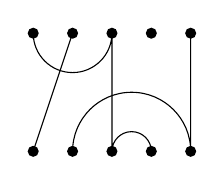
\begin{tikzpicture}[scale=0.5]
\foreach \x in {1,...,5}
	{\fill[black] (\x,3) circle (4pt);
	\fill[black] (\x,0) circle (4pt);}
	\draw (1,3) arc (-180:0:1) -- (3,0) arc (180:0:0.5);
	\draw (2,3)--(1,0);
	\draw (2,0) arc (180:0:1.5) -- (5,3);
\end{tikzpicture}\hspace{1cm}
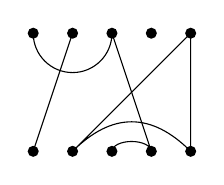
\begin{tikzpicture}[scale=0.5]
\foreach \x in {1,...,5}
	{\fill[black] (\x,3) circle (4pt);
	\fill[black] (\x,0) circle (4pt);}
	\draw (1,3) arc (-180:0:1) -- (4,0) arc (0:180:0.5 and 0.25);
	\draw (2,3)--(1,0);
	\draw (2,0) .. controls (3,1) and (4,1) .. (5,0) -- (5,3) -- (2,0);
\end{tikzpicture}\hspace{1cm}
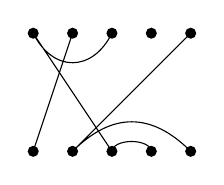
\begin{tikzpicture}[scale=0.5]
\foreach \x in {1,...,5}
	{\fill[black] (\x,3) circle (4pt);
	\fill[black] (\x,0) circle (4pt);}
	\draw (3,3) .. controls (2.5,2) and (1.5,2) .. (1,3) -- (3,0)
 arc (180:0:0.5 and 0.25);
	\draw (2,3)--(1,0);
	\draw (5,0) .. controls (4,1) and (3,1) .. (2,0) -- (5,3);
\end{tikzpicture}
%\]
\end{gather*}
\end{exam}
	
	
	
\begin{exam}
In the following example, the diagram on the right-hand side of the
equality is obtained by stacking the two diagrams on the left of the
equality on top of each other (with the leftmost diagram on top) and
removing the singleton from the middle of the diagram (at the expense
of multiplication by the parameter $\delta^1$).
\[
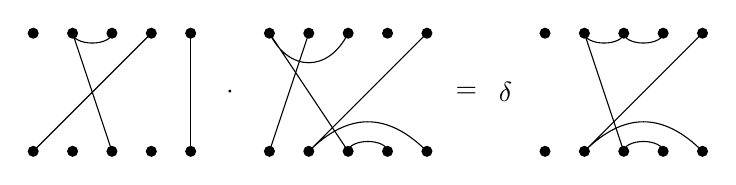
\begin{tikzpicture}[scale=0.5]
\foreach \x in {1,...,5,7,8,...,11,14,15,...,18}
	 {\fill[black] (\x,0) circle (4pt);
	 \fill[black] (\x,3) circle (4pt);}
	 \draw (3,3) arc (0:-180:0.5 and 0.25) -- (3,0);
 \draw (4,3)--(1,0);\draw (5,3)--(5,0);
	\draw (6,1.5) node {$\cdot$};
	\draw (9,3) .. controls (8.5,2) and (7.5,2) .. (7,3) -- (9,0)
 arc (180:0:0.5 and 0.25);
	\draw (8,3)--(7,0);
	\draw (11,0) .. controls (10,1) and (9,1) .. (8,0) -- (11,3);
	\draw (12,1.5) node {$=$};\draw (13,1.5) node {$\delta$};
	\draw (18,0) .. controls (17,1) and (16,1) .. (15,0) -- (18,3);
	\draw (17,3) arc (0:-180:0.5 and 0.25)
 arc (0:-180:0.5 and 0.25) -- (16,0) arc (180:0:0.5 and 0.25);
\end{tikzpicture}
\]
\end{exam}
	
The half partition algebra $\Ptn_{r+\half}(\delta)$, introduced in
\cite{Martin:2000}, is the subalgebra of $\Ptn_{r+1}(\delta)$ spanned
by diagrams such that vertex $r+1$ is connected to vertex $(r+1)'$.

By specialising the parameter $\delta$ to $n$, we obtain a linear
representation of $\Ptn_r(n)^{\op}$, defined as follows. Let $I(n,r) =
\{1, \dots, n\}^r$ be the set of multi-indices of length $r$. To
simplify the notation, we often write
\[
 \text{$i_1 \cdots i_r$ instead of $(i_1, \dots, i_r)$}
\]
for an element of $I(n,r)$. Elements of $I(n,r)$ can also be written
as $i_{1'} \cdots i_{r'}$ or $(i_{1'}, \dots, i_{r'})$. Connected
components of a diagram are called \emph{blocks}; they correspond to
the subsets of the underlying set partition. Following~\cite{HR-2005},
we define a scalar $(d)^{i_1 \cdots i_r}_{i_{1'} \cdots i_{r'}} \in
\Bbbk$, for a diagram $d$ and any $i_1 \cdots i_r$, $i_{1'} \cdots
i_{r'}$ in $I(n,r)$, by
\[
(d)^{i_1 \cdots i_r}_{i_{1'} \cdots i_{r'}} = 
\begin{cases}
 1 & \text{if } i_\alpha = i_\beta \text{ whenever } \alpha \ne
 \beta \text{ are in the same block of } d,\\ 
 0 & \text{otherwise}.
\end{cases}
\]
Here, the indices $\alpha,\beta$ may be primed or unprimed. The
diagram $d$ acts on $\V^{\otimes r}$, on the right, by the rule
\begin{equation}\label{eq:Ptn-action}
(\bv_{i_1} \otimes \cdots \otimes \bv_{i_r})^d = \sum_{i_{1'} \cdots
 i_{r'}} (d)^{i_1 \cdots i_r}_{i_{1'} \cdots i_{r'}} \, (\bv_{i_{1'}}
 \otimes \cdots \otimes \bv_{i_{r'}})
\end{equation}
extended linearly. Note that if $d \in \Sym_r$ is a permutation
diagram, then $d$ acts by the usual place-permutation action. Extended
linearly, this action defines a linear representation $\Ptn_r(n)^{\op}
\to \End_\Bbbk(\V^{\otimes r})$. The commuting actions define a
$(\Bbbk W_n, \Ptn_r(n))$-bimodule structure on $\V^{\otimes r}$. By
identifying $\V^{\otimes r}$ with $\V^{\otimes r} \otimes \bv_n
\subset \V^{\otimes (r+1)}$, by restriction $\V^{\otimes r}$ may also
be regarded as a $(\Bbbk W_{n-1}, \Ptn_{r+\half}(n))$-bimodule, where
$W_{n-1}$ is identified with the subgroup of $W_n$ consisting of the
permutations fixing $n$.

Because the actions commute, the representations $\Bbbk W_n
\to \End_\Bbbk(\V^{\otimes r})$, $\Ptn_r(n) \to \End_\Bbbk(\V^{\otimes
 r})$ induce $\Bbbk$-algebra homomorphisms
\begin{equation}\label{eq:induced-homs}
\begin{aligned}
 \Phi_{n,r}&: \Bbbk W_n \to \End_{\Ptn_r(n)}( \V^{\otimes r} ),\\
 \Psi_{n,r}&: \Ptn_r(n)^{\op} \to \End_{W_n}( \V^{\otimes r} )
\end{aligned}
\end{equation}
into the respective centraliser algebras. Similarly, by restriction we
have induced $\Bbbk$-algebra homomorphisms
\begin{equation}\label{eq:induced-homs-half}
\begin{aligned}
 \Phi_{n,r+\half}&: \Bbbk W_{n-1}
 \to \End_{\Ptn_{r+\half}(n)}(\V^{\otimes r} ), \\ \Psi_{n,r+\half}&:
 \Ptn_{r+\half}(n)^{\op} \to \End_{W_{n-1}}( \V^{\otimes r} ).
\end{aligned}
\end{equation}
Schur--Weyl duality is equivalent to the surjectivity of these induced
homomorphisms. As noted above, the combinatorial argument given in~\cite[Thm.~3.6]{HR-2005}, which works over any commutative ring
$\Bbbk$, proves the surjectivity of the maps $\Psi_{n,r}$,
$\Psi_{n,r+\half}$. Indeed, the partition algebra was originally
defined with that property in mind.

Thus, we only need to prove the surjectivity of the induced maps
$\Phi_{n,r}$, $\Phi_{n,r+\half}$ defined in~\eqref{eq:induced-homs}, \eqref{eq:induced-homs-half}.



\section{Generalised doubly-stochastic matrices}%\noindent
\label{sec:GDS}%
We denote the entry in the $i$th row and $j$th column of a matrix
$\bM$ by $m^i_j$, and write $\bM=(m^i_j)$. In this paper, we will
always follow this convention of using bold letters for matrices and
lower case letters for their entries. 
It will be convenient to employ the following terminology; see \eg \cite{Brualdi, Johnsen, Gibson, Lai}.

\begin{defi}\label{def:GDS}
 An $n \times n$ matrix $\bM = \big( m^i_j \big)_{i,j = 1, \dots, n}$
 is \emph{generalised doubly-stochastic} (GDS) if there is some $s =
 s(\bM)$ in $\Bbbk$ such that both:
 \begin{enumerate}[label=(\alph*)]
 \item $\sum_{j=1}^n m^i_j = s$, for all $i=1, \dots, n$, and
 \item $\sum_{i=1}^n m^i_j = s$, for all $j = 1, \dots, n$. 
 \end{enumerate}
\end{defi}

In other words, $\bM$ is GDS if there is a common value for all its
row and column sums. 

\begin{lemm}\label{lem:GDS}
 Assume that $n > 1$. An $n \times n$ matrix $\bM$ over the ring
 $\Bbbk$ is GDS if and only if $\bM$ commutes with the matrix $\bJ_n =
 (1)_{i,j=1,\dots, n}$ of all ones.
\end{lemm}

\begin{proof}
The matrix $\bJ_n \bM$ is the $n \times n$ matrix with the column sum
$\co_i(\bM) := \sum_j m^i_j$ in each entry of the $i$th column. On the
other hand, $\bM \bJ_n$ is the $n \times n$ matrix with the row sum
$\ro_j(\bM) := \sum_i m^i_j$ in each entry of the $j$th row. So $\bM$
commutes with $\bJ_n$ if and only if $\co_i(\bM) = \ro_j(\bM)$ for all
$i,j = 1, \dots, n$. Since $n > 1$, it follows that this is so if and
only if all the row and column sums have a common value.
\end{proof}

Let $\bM$ be a generalised doubly-stochastic matrix. 
If $\bM$ is identified with the $\Bbbk$-linear endomorphism of $\V$
defined by $\bv_j \mapsto \sum_i m^i_j \, \bv_i$, then $s(\bM)$ is an
eigenvalue for the eigenvector $\bv_1 + \cdots + \bv_n$. The proof is
easy. This observation leads to the following characterisation of GDS
operators, where GDS operators on $\V$ are defined to be linear
operators whose matrices with respect to the basis $\{\bv_1, \dots,
\bv_n\}$ are GDS.

\section{Description of the invariants \texorpdfstring{$\E_\Bbbk(n,r)$}{Ek (n,r)}}%
\label{sec:invariants}%\noindent
To ease the notation, we henceforth put $\E_\Bbbk(n,r)
= \End_{\Ptn_r(n)}(\V^{\otimes r})$. Similarly, we set
$\E_\Bbbk(n,r+\fhalf) = \End_{\Ptn_{r+\half}(n)}(\V^{\otimes r})$. The
purpose of this section is to describe $\E_\Bbbk(n,r)$; a description
of $\E_\Bbbk(n,r+\fhalf)$ will be given in the next section.

We introduce some additional notation. For each multi-index $\bi =
i_1\cdots i_r$ in $I(n,r)$, $\sigma$ in $\Sym_r$, and $w$ in $W_n$, we
set
\[
 \bi^\sigma = (i_1\cdots i_r)^\sigma = i_{1 \sigma^{-1}} \cdots
 i_{r \sigma^{-1}}, \quad w \bi = w(i_1 \cdots i_r) = w(i_1) \cdots w(i_r).
\] 
The assignment $(\bi , \sigma) \mapsto \bi^\sigma$ defines a right
action (the place-permutation action) of the symmetric group $\Sym_r$
on the set $I(n,r)$; the assignment $(w,\bi) \mapsto w \bi$ defines a
left action of $W_n$ on $I(n,r)$. These left and right actions on
$I(n,r)$ commute: $(w\bi)^\sigma = w(\bi^\sigma)$, for all $w \in
W_n$, $\sigma \in \Sym_r$. Set:
\begin{equation}
 \bv_\bi = \bv_{i_1} \otimes \cdots \otimes \bv_{i_r}.
\end{equation}
Then the basis of $\V^{\otimes r}$ given in~\eqref{eq:TS-basis} is
$\{\bv_\bi: \bi \in I(n,r)\}$, and the commuting actions of $W_n$ and
$\Sym_r$ on $\V^{\otimes r}$ considered in Section~\ref{sec:bimodules}
are given by the rules $(w, \bv_\bi) \mapsto \bv_{w\bi}$ and
$(\bv_\bi, \sigma) \mapsto \bv_{\bi^\sigma}$.

Orbits for the left action of $W_n$ on $I(n,r)$ are called
\emph{value-types} and may be identified with set partitions of $\{1,
\dots, r\}$. The subsets in the value-type $\vt(\bi) = \Lambda$ of
$\bi = i_1 \cdots i_r$ record the positions at which the distinct
values that appear are constant. More precisely, we make the following
definition.

\begin{defi}\label{def:value-type}
 Let $\bi = i_1 \cdots i_r \in I(n,r)$ be given. For each $v =
 1, \dots, n$, let $\Lambda'_v$ be the set of all positions
 $\alpha = 1, \dots, r$ for which $i_\alpha = v$. Then $\{1, \dots,
 r\} = \bigcup_{v=1}^n \Lambda'_v$. Discard any empty $\Lambda'_v$ to
 obtain the set partition $\Lambda = \{ \Lambda'_v : \Lambda'_v \ne
 \emptyset\}$ which defines $\vt(\bi)$. Let $\ell(\Lambda)$ be the
 number of non-empty subsets in $\Lambda$.
\end{defi}

For example, the multi-index $\bi = abbcabc$ (for distinct elements
$a,b,c \in \{1, \dots, n\}$) has value-type $\vt(\bi) = \{\{1,5\},
\{2,3,6\}, \{4,7\}\}$.

Recall that orbits for the right action of $\Sym_r$ on $I(n,r)$ are
called \emph{weights} and may be identified with weak compositions of
$r$ of length at most $n$. To be precise, the weight $\wt(\bi)$ of a
multi-index $\bi = i_1 \cdots i_r$ is the composition $\wt(\bi) =
(\mu_1, \dots, \mu_n)$ where for each value $v = 1, \dots, n$ the
statistic $\mu_v$ counts the number of positions $\alpha = 1, \dots,
r$ such that $i_\alpha = v$. In other words, $\mu_v = |\Lambda'_v|$
for each $v = 1, \dots, n$.

We also need to consider the set $\Omega(n,r)$ of orbits for the right
action of $\Sym_r$ on $I(n,r) \times I(n,r)$ defined by
$(\bi, \bj)^\sigma = (\bi^\sigma, \bj^\sigma)$.

In order to describe the invariants $\End_{\Ptn_r(n)}(\V^{\otimes r})$
it suffices to consider a set of generators. Halverson and Ram~\cite{HR-2005} 
showed that $\Ptn_r(\delta)$ is generated by the
diagrams:
\[
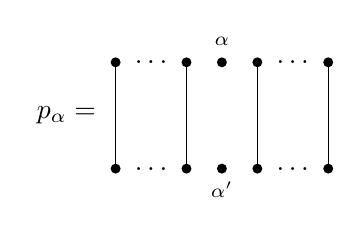
\begin{tikzpicture}[scale=0.45]
	\draw (-1,1.5) node {$p_\alpha=\quad$};
	\foreach \x in {0,2,3,4,6}
	{\fill[black] (\x,0) circle (4pt);
	\fill[black] (\x,3) circle (4pt);}
	\foreach \x in {0,2,4,6}
	{\draw (\x,3)--(\x,0);}
	\draw (3,3.6) node {$\scriptstyle\alpha$};
	\draw (3,-0.6) node {$\scriptstyle\alpha'$};
\draw (1,0) node {$\ldots$};\draw (1,3) node {$\ldots$};
\draw (5,0) node {$\ldots$};\draw (5,3) node {$\ldots$};
\end{tikzpicture}
\hspace{0.5in}
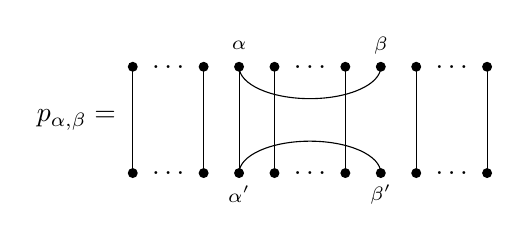
\begin{tikzpicture}[scale=0.45]
	\draw (-1.2,1.5) node {$p_{\alpha,\beta}=\quad$};
	\foreach \x in {0,2,3,4, 5.5+.5,6.5+.5,8,10}
	{\fill[black] (\x,0) circle (4pt);
	\fill[black] (\x,3) circle (4pt);}
	\foreach \x in {0,2,4, 5.5+.5,7.5+.5,10}%{1,2,4,5,7}
	{\draw (\x,3)--(\x,0);}
	\draw (3,3)--(3,0); \draw (3,3) arc (0:180:-2 and -0.9) ;
 \draw (3,0) arc (0:180:-2 and 0.9) ;
	\draw (3,3.6) node {$\scriptstyle\alpha$};\draw (7,3.6)
 node {$\scriptstyle\beta$};
	\draw (3,-0.6) node {$\scriptstyle\alpha'$};\draw (7,-0.6)
 node {$\scriptstyle\beta'$};
\draw (1,3) node {$\ldots$};\draw (1,0) node {$\ldots$};
\draw (5,3) node {$\ldots$};\draw (5,0) node {$\ldots$};
\draw (9,3) node {$\ldots$};\draw (9,0) node {$\ldots$};
\end{tikzpicture}
\]
\[
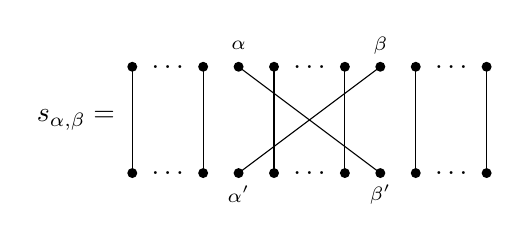
\begin{tikzpicture}[scale=0.45]
	\draw (-1.2,1.5) node {$s_{\alpha,\beta}=\quad$};
	\foreach \x in {0,2,3,4, 5.5+.5,6.5+.5,8,10}
	{\fill[black] (\x,0) circle (4pt);
	\fill[black] (\x,3) circle (4pt);}
	\foreach \x in {0,2,4, 5.5+.5,7.5+.5,10}%{1,2,4,5,7}
	{\draw (\x,3)--(\x,0);}
	\draw (3,3)--(7,0);\draw (7,3)--(3,0);
	\draw (3,3.6) node {$\scriptstyle\alpha$};\draw (7,3.6)
 node {$\scriptstyle\beta$};
	\draw (3,-0.6) node {$\scriptstyle\alpha'$};\draw (7,-0.6)
 node {$\scriptstyle\beta'$};
\draw (1,3) node {$\ldots$};\draw (1,0) node {$\ldots$};
\draw (5,3) node {$\ldots$};\draw (5,0) node {$\ldots$};
\draw (9,3) node {$\ldots$};\draw (9,0) node {$\ldots$};
\end{tikzpicture}\hspace{0.5cm}
\]
where $1 \leq \alpha<\beta \leq r$. In fact, $\Ptn_r(\delta)$ is
generated by the usual Coxeter generators $s_{\alpha,\alpha+1}$ for
$\alpha = 1, \dots, r-1$ along with just one $p_\alpha$ and one
$p_{\alpha,\beta}$.

Let $\GG_r(n)$, $\HH_r$, $\Bbbk\Sym_r$ be the subalgebras of
$\Ptn_r(n)$ respectively generated by the $p_\alpha$,
$p_{\alpha,\beta}$, and $s_{\alpha,\beta}$ pictured above. Note that
$\HH_r$ is independent of $n$. We shall separately consider the
centraliser algebras of these three subalgebras:
\[
%\begin{gather*}
G_\Bbbk(n,r) = \End_{\GG_r(n)}(\V^{\otimes r}), \quad
H_\Bbbk(n,r) = \End_{\HH_r} (\V^{\otimes r}), \quad %\\ 
S_\Bbbk(n,r) = \End_{\Sym_r} (\V^{\otimes r}).
%\end{gather*}
\]
Then we have $\E_\Bbbk(n,r) = G_\Bbbk(n,r) \cap H_\Bbbk(n,r) \cap
S_\Bbbk(n,r)$. Note that $S_\Bbbk(n,r)$ is the classical Schur algebra
appearing in~\cite{Green:book}. Furthermore, we have
$\HH_1=\Bbbk\Sym_1=\Bbbk$ and thus
$H_\Bbbk(n,1)=S_\Bbbk(n,1)=\End_\Bbbk(\V)$, which means that
$\E_\Bbbk(n,1) = G_\Bbbk(n,1)$. By Lemma~\ref{lem:GDS}, the algebra
$G_\Bbbk(n,1)$ coincides with the set of $n \times n$ GDS matrices
considered in Section~\ref{sec:GDS}.

Henceforth, we write $\Mat_{I(n,r)}(\Bbbk)$ for the set of $n^r \times
n^r$ matrices over $\Bbbk$, with rows and columns indexed by the set
$I(n,r)$ according to the lexicographic ordering. We always identify
the matrix $\bA = (a^\bi_\bj)$ with the $\Bbbk$-linear endomorphism of
$\V^{\otimes r}$ defined on basis elements by $\bv_\bj \mapsto
\sum_{\bi \in I(n,r)} a^{\bi}_{\bj} \, \bv_{\bi}$.

\begin{prop}\label{prop:GHS}
 Let $G_\Bbbk(n,r)$, $H_\Bbbk(n,r)$, and $S_\Bbbk(n,r)$ be the
 subalgebras of $\End_\Bbbk( \V^{\otimes r} )$ consisting of
 the endomorphisms commuting with the action of all the $p_\alpha$,
 $p_{\alpha,\beta}$, and $s_{\alpha,\beta}$ respectively. Let $\bA =
 ( a^{\bi}_{\bj} ) \in \Mat_{I(n,r)}(\Bbbk)$. Then
\begin{enumerate}[label=(\alph*)]
\item\label{prop3.2_a} $\bA$ belongs to $G_\Bbbk(n,r)$ if and only if for each place
 $\alpha = 1, \dots, r$ and for each fixed $\bp = i_1 \cdots
 i_{\alpha-1} i_{\alpha+1}\cdots i_r$, $\bq = j_1 \cdots j_{\alpha-1}
 j_{\alpha+1} \cdots j_r$ in $I(n,r-1)$ there is some scalar
 $b^\bp_\bq(\alpha)$ in $\Bbbk$ such that
 \begin{align*}
 \sum_{i = 1}^n a^{i_1 \cdots i_{\alpha-1}\, i\, i_{\alpha+1}
 \cdots i_r}_{j_1 \cdots j_{\alpha-1}\, j\, j_{\alpha+1} \cdots
 j_r} &= b^\bp_\bq(\alpha), \text{ for any } j = 1, \dots, n
 \\ \intertext{ and} \sum_{j = 1}^n a^{i_1 \cdots i_{\alpha-1}\,
 i\, i_{\alpha+1} \cdots i_r}_{j_1 \cdots j_{\alpha-1}\, j\,
 j_{\alpha+1} \cdots j_r} &= b^\bp_\bq(\alpha), \text{ for any }
 i = 1, \dots, n.
 \end{align*}

\item\label{prop3.2_b} $\bA$ belongs to $H_\Bbbk(n,r)$ if and only if $\bA$ preserves
 value-type, in the sense: $a^{\bi}_{\bj} = 0$ for all pairs
 $(\bi,\bj) \in I(n,r) \times I(n,r)$ such that $\vt(\bi) \ne
 \vt(\bj)$.
 
\item\label{prop3.2_c} $\bA$ belongs to $S_\Bbbk(n,r)$ if and only if $\bA$ is constant
 on each place-permutation orbit $\Orb$ in $\Omega(n,r)$, \ie if
 $a^\bi_\bj = a^\bk_\bl$ whenever $(\bi,\bj)$ and $(\bk,\bl)$ are in
 the same orbit $\Orb \in \Omega(n,r)$.
\end{enumerate}
\end{prop}

\begin{proof}
%
\ref{prop3.2_a}~Suppose that $1 \le \alpha \le r$. By the definition in equation~\eqref{eq:Ptn-action}, the matrix $\Psi_{n,r}(p_{\alpha})$ representing $p_{\alpha}$ with respect to the basis $\{\bv_\bi : \bi \in I(n,r)\}$ has the form
\[
\big( \delta_{i_1,j_1} \cdots \delta_{i_{\alpha-1}, j_{\alpha-1}}
\delta_{i_{\alpha+1}, j_{\alpha+1}} \cdots \delta_{i_r, j_r} \big)_{\bi,\bj
 \in I(n,r) \times I(n,r)} \, .
\]
More succinctly, the matrix can be written as $(\bI_n)^{\otimes
 \alpha-1} \otimes \bJ_n \otimes (\bI_n)^{\otimes r-\alpha}$, where
$\bJ_n$ is the $n \times n$ matrix defined in Section~\ref{sec:GDS}. It follows immediately from Lemma~\ref{lem:GDS} that
the commutant $\End_{p_\alpha}(\V^{\otimes r})$ of $p_\alpha$
is the set of endomorphisms satisfying the displayed condition in part~\ref{prop3.2_a} of the proposition. Thus, the centraliser $G_\Bbbk(n,r)$ of all
the $p_\alpha$ for $1 \le \alpha \le r$ is the set of endomorphisms
satisfying the condition for all $\alpha$. This proves part~\ref{prop3.2_a}.
 
\ref{prop3.2_b}~Suppose that $1 \le \alpha < \beta \le r$. By~\eqref{eq:Ptn-action}, the matrix $\Psi_{n,r}(p_{\alpha,\beta})$
representing $p_{\alpha,\beta}$ with respect to the basis $\{\bv_\bi :
\bi \in I(n,r)\}$ is
\[
\big( \delta_{i_{1},j_{1}} \cdots \delta_{i_{\alpha-1},j_{\beta-1}}
\delta_{i_\alpha, i_\beta, j_\alpha, j_\beta} \delta_{i_{\alpha+1},j_{\beta+1}} \cdots
\delta_{i_r,j_r} \big)_{(\bi,\bj) \in I(n,r) \times I(n,r)}.
\]
Here $\delta_{i_\alpha, i_\beta, j_\alpha, j_\beta} = \delta_{i_\alpha,
 i_\beta} \delta_{i_\alpha, j_\alpha} \delta_{i_\alpha, j_\beta}$ is a
generalised Kronecker delta symbol, which is 1 if
$i_\alpha=i_\beta=j_\alpha=j_\beta$ and 0 otherwise. So the matrix
$\Psi_{n,r}(p_{\alpha,\beta})$ is a diagonal matrix with
$(\bi,\bi)$-entry equal to
\[
\begin{cases}
 1 & \text{if } i_\alpha
 = i_\beta ,\\
 0 & \text{otherwise},
\end{cases}
\]
for $\bi = i_1 \cdots i_r$ in $I(n,r)$. If we reorder $I(n,r)$ so
that all the nonzero diagonal entries come before the zero ones, then
the matrix $\Psi_{n,r}(p_{\alpha,\beta})$ has the block form
 \[
\setlength{\arraycolsep}{4pt}
 \left[\begin{array}{c|c} {\bI} & \bzero \\ \hline \bzero &
 \bzero\end{array}\right]
 \]
and an easy calculation with block matrices shows that the commutant
$\End_{p_{\alpha,\beta}}(\V^{\otimes r})$ of $p_{\alpha,\beta}$
consists of all block matrices of the form
 \[
\setlength{\arraycolsep}{4pt}
 \left[\begin{array}{c|c}
 \bA & \bzero \\ \hline \bzero & \bB
 \end{array}\right]
 \]
where $\bA, \bB $ are arbitrary matrices (of the relevant sizes). So
$p_{\alpha,\beta}$ sends all $\bv_\bi$ satisfying the condition
$i_\alpha = i_\beta$ to a linear combination of $\bv_\bj$ such that
$j_\alpha = j_\beta$ and sends the $\bv_\bi$ satisfying $i_\alpha \ne
i_\beta$ to a linear combination of $\bv_\bj$ such that $j_\alpha \ne
j_\beta$.

It follows that the centraliser algebra $H_\Bbbk(n,r)$, which is the
intersection of the commutants of the various $p_{\alpha,\beta}$ for
$1 \le \alpha < \beta \le r$, is the algebra of all value-type
preserving endomorphisms. This proves part~\ref{prop3.2_b}.

\ref{prop3.2_c}~The proof of part~\ref{prop3.2_c} is well known and can be found, for instance, in~\cite{Green:book}.
\end{proof}




\begin{defi}\label{def:slices}
Let $\bi = i_1 \cdots i_r$, $\bj = j_1 \cdots j_r$ be given
multi-indices. Suppose that $\alpha \in \{1, \dots, r\}$ is a
place. The row and column $\alpha$-\emph{slices} of $\bA$ determined
by $(\bi,\bj)$ are respectively the $n$-vectors
 \[
 \big( a^{i_1\cdots i_{\alpha-1} \,i\, i_{\alpha+1}\cdots
 i_r}_{j_1\cdots j_{\alpha-1} \, j_\alpha\, j_{\alpha+1}\cdots
 j_r}\big)_{i = 1, \dots, n} \quad \text{ and } \quad \big(
 a^{i_1\cdots i_{\alpha-1} \,i_\alpha\, i_{\alpha+1}\cdots
 i_r}_{j_1\cdots j_{\alpha-1} \,j\, j_{\alpha+1}\cdots j_r}
 \big)_{j = 1, \dots, n} .
 \]
We denote these vectors respectively by the suggestive shorthand
notations
 \[
 a^{i_1\cdots i_{\alpha-1} \,*\, i_{\alpha+1}\cdots i_r}_{j_1\cdots
 j_{\alpha-1} \, j_\alpha\, j_{\alpha+1}\cdots j_r} \qand a^{i_1\cdots
 i_{\alpha-1} \,i_\alpha\, i_{\alpha+1}\cdots i_r}_{j_1\cdots
 j_{\alpha-1} \,*\, j_{\alpha+1}\cdots j_r} \, .
 \]
Putting a $\sum$ symbol in front of a slice implies a sum over
the elements of the slice. We also extend this notation in the
obvious way to allow two or more $*$s to appear; we call them
\emph{double slices}, \etc
\end{defi}

Here are some basic properties of invariants in $\E_\Bbbk(n,r)$, for
$r \ge 2$. (If $r=1$, invariants in $\E_\Bbbk(n,r)$ are just $n
\times n$ GDS matrices; see Section~\ref{sec:GDS}.)

\begin{prop}\label{prop:inv-properties}
 Suppose that $r \ge 2$ and that $\bA$ is an element of
 $\E_\Bbbk(n,r)$. Then:
 \begin{enumerate}[label=(\alph*)]
 \item\label{prop3.4_a} For any $\bp$, $\bq \in I(n,r-1)$, the scalars
 $b^\bp_\bq(\alpha)$ appearing in Proposition
~\ref{prop:GHS}\ref{prop3.2_a} are
 independent of $\alpha$. That is, all the slice sums determined by
 $\bp, \bq$ have the same value $b^\bp_\bq$.
 \item\label{prop3.4_b} For any $\bp$, $\bq \in I(n,r-1)$, let $\bA^\bp_\bq$ be the $n
 \times n$ block $\bA^\bp_\bq = (a^{\bp\, i}_{\bq\, j})_{i,j = 1,
 \dots, n}$. Then $\bA^\bp_\bq$ is GDS, with common row and
 column sums equal to $b^\bp_\bq$.
 \item\label{prop3.4_c} If $\bi = i_1 \cdots i_r$, $\bj = j_1 \cdots j_r$ are in
 $I(n,r)$ and $\vt(\bi) \ne \vt(\bj)$ then $a^\bi_\bj = 0$.
 \item\label{prop3.4_d} If $\bi = i_1 \cdots i_r$, $\bj = j_1 \cdots j_r$ are in
 $I(n,r)$, $\vt(\bi) = \vt(\bj)$, and $i_r$ appears in $\bp = i_1
 \cdots i_{r-1}$, then $j_r$ also appears in the same place in $\bq
 = j_1 \cdots j_{r-1}$, and $a^\bi_\bj = b^\bp_\bq$.
 \end{enumerate}
\end{prop}

\begin{proof}
\ref{prop3.4_a}~Since $\E_\Bbbk(n,r)$ is the intersection of $G_\Bbbk(n,r)$,
$H_\Bbbk(n,r)$, and $S_\Bbbk(n,r)$ it is clear that $\bA$ must be
constant on place-permutation orbits, by Proposition~\ref{prop:GHS}\ref{prop3.2_c}. This immediately implies that its slice sums are
independent of $\alpha$.

\ref{prop3.4_b}~This follows from part~\ref{prop3.4_a}. Explicitly, for any $\alpha = 1,
\dots, r$ and any given $\bp = i_1 \cdots i_{\alpha-1} i_{\alpha+1}
\cdots i_r$, $\bq = j_1 \cdots j_{\alpha-1} \, j_{\alpha+1} \cdots
j_r$ in $I(n,r-1)$, part~\ref{prop3.4_a} says that there exists a scalar
$b^\bp_\bq$ in $\Bbbk$ such that
\[
\sum a^{i_1\cdots i_{\alpha-1} \,*\, i_{\alpha+1}\cdots
 i_r}_{j_1\cdots j_{\alpha-1} \, j \, j_{\alpha+1}\cdots j_r} =
b^\bp_\bq \qand \sum a^{i_1\cdots i_{\alpha-1} \, i \,
 i_{\alpha+1}\cdots i_r}_{j_1\cdots j_{\alpha-1} \,*\,
 j_{\alpha+1}\cdots j_r} = b^\bp_\bq
\]
for any $i,j = 1, \dots, n$. Part~\ref{prop3.4_b} is the particular case where
$\bp = i_1 \cdots i_{r-1}$, $\bq = j_1 \cdots j_{r-1}$.

\ref{prop3.4_c}~This is the same as part~\ref{prop3.4_b} of Proposition~\ref{prop:GHS}, repeated
here for the sake of convenience.

\ref{prop3.4_d}~This follows from parts~\ref{prop3.4_b} and~\ref{prop3.4_c}. By part~\ref{prop3.4_c}, under these hypotheses, all terms except $a^{\bp\,i_r}_{\bq\,j_r}$ of the slice
sum $\sum a^{\bp\,i_r}_{\bq\,*} = b^{\bp}_{\bq}$ must be zero.
\end{proof}

\begin{defi}\label{def:restr}
 Assume that $r \ge 1$. Let $\bA \in \E_\Bbbk(n,r)$ be given. For
 any $\bp$, $\bq \in I(n,r-1)$ let $b^\bp_\bq$ be the common value of
 the slice sums in $\bA$ indexed by $\bp, \bq$. (This is a single
 scalar if $r=1$.) The matrix $\bB = (b^\bp_\bq)_{\bp,\bq \in
 I(n,r-1)}$ in $\Mat_{I(n,r-1)}(\Bbbk)$ is the \emph{restriction}
 of $\bA$. We write $\rho(\bA) = \bB$ for the restriction.
\end{defi}

Proposition~\ref{prop:inv-properties}\ref{prop3.4_b} says that the invariant
$\bA$ is obtained by ``blowing up'' its restriction $\bB = \rho(\bA)$
by a process which replaces each matrix entry $b^\bp_\bq$ of $\bB$ by
an $n \times n$ GDS matrix with row and column sums equal to
$b^\bp_\bq$. Of course, $\bA$ must also be invariant under
place-permutations, so blowing up is not the only consideration.

\begin{prop}\label{prop:restr-is-invariant}
 Let $r \ge 1$, and suppose that $\bA \in \E_\Bbbk(n,r)$. Then the
 restriction $\rho(\bA)$ belongs to $\E_\Bbbk(n,r-1)$. Thus, $\rho$
 is a $\Bbbk$-linear map from $\E_\Bbbk(n,r)$ into $\E_\Bbbk(n,r-1)$.
\end{prop}

\begin{proof}
Set $\bB = \rho(\bA)$. If $r=1$ then $\bB$ is just a scalar and there
is nothing to prove, since $\E_\Bbbk(n,0) = \Bbbk$. For the moment, we
assume that $r=2$. Given any $i_1i_2 \in I(n,2)$, we compute the
double-slice sum $\sum a^{i_1i_2}_{**}$ two ways, by applying the
independence in Proposition~\ref{prop:inv-properties} and changing
the order of summation:
\begin{align*}
\sum a^{i_1i_2}_{**} &= \sum_{j=1}^n \sum_{j'=1}^n a^{i_1i_2}_{jj'} =
\sum_{j=1}^n b^{i_1}_j = \sum b^{i_1}_*\\
&= \sum_{j'=1}^n \sum_{j=1}^n a^{i_1i_2}_{jj'} =
\sum_{j=1}^n b^{i_2}_{j'} = \sum b^{i_2}_* .
\end{align*}
Thus all the row sums in $\bB$ have a common value. Similarly, by
considering the double-slice sum $\sum a^{**}_{j_1j_2}$ we see that
$\sum b^*_{j_1} = \sum b^*_{j_2}$, for arbitrary $j_1j_2$ in $I(n,2)$,
so all the column sums in $\bB$ have a common value. Finally, for
arbitrary $i_1, j_2 = 1, \dots, n$ we compute the mixed-double-slice
sum $\sum a^{i_1*}_{*j_2}$ two ways:
\begin{align*}
\sum a^{i_1*}_{*j_2} &= \sum_{i=1}^n \sum_{j=1}^n a^{i_1i}_{jj_2} =
\sum_{i=1}^n b^{i}_{j_2} = \sum b^{*}_{j_2}\\
&= \sum_{j=1}^n \sum_{i=1}^n a^{i_1i}_{jj_2} =
\sum_{j=1}^n b^{i_1}_{j} = \sum b^{i_1}_* .
\end{align*}
Thus $\sum b^{*}_{j_2} = \sum b^{i_1}_{*}$. This shows that all the
row sums are equal to all the column sums in $\bB$. In other words,
$\bB$ is GDS, and thus belongs to $\E_\Bbbk(n,1)$. This proves the
result in case $r=2$.

Now assume that $r>2$. We need to show that $\bB$ satisfies the
conditions of Proposition~\ref{prop:GHS}\ref{prop3.2_a}--\ref{prop3.2_c}. It is easy to see
that conditions~\ref{prop3.2_b},~\ref{prop3.2_c}~hold for $\bB$ since they hold for
$\bA$. Then calculations similar to the above (and place-permutation
invariance) show that $\bB$ satisfies the slice-sum equations in part~\ref{prop3.2_a}. Thus $\bB$ belongs to $\E_\Bbbk(n,r-1)$ as claimed.
\end{proof}

Going forward, we will often regard a given $\bA = (a^{i_1
 \cdots i_r}_{j_1 \cdots j_r})_{i_1 \cdots i_r, j_1 \cdots j_r \in
 I(n,r)}$ in $\E_\Bbbk(n,r)$ as the $n \times n$ block matrix
\begin{equation}\label{eq:blocks}
\bA = (\bA^i_j)_{i,j = 1, \dots,n} = 
\begin{bmatrix}
 \bA^1_1 & \cdots & \bA^1_n \\
 \vdots & \ddots & \vdots \\
 \bA^n_1 & \cdots & \bA^n_n
\end{bmatrix}
\end{equation}
where each block $\bA^i_j$ is defined by $\bA^i_j = (a^{i\, i_2 \cdots
 i_r}_{j\, j_2 \cdots j_r})_{i_2 \cdots i_r, j_2 \cdots j_r \in
 I(n,r-1)}$.

\begin{rema}\label{rmk:block-sums}
The block notation just introduced provides a convenient description
of the restriction map. Given $\bA$ in $\E_\Bbbk(n,r)$, we have
\[
\rho(\bA) = \textstyle \sum \bA^i_* = \sum \bA^*_j
\]
for any $i,j$. That is, the restriction $\bB=\rho(\bA)$ is the common
value of the block row and column sums in the block matrix~\eqref{eq:blocks}.
\end{rema}

\begin{exam}\label{ex:n23-r2-inv}
We now illustrate how, using only the value-type condition of
Proposition~\ref{prop:GHS}\ref{prop3.2_b} we can obtain general forms for the
invariants $\E_\Bbbk(n,r)$ for small values of $n$ and $r$ (we will
use blank entries to denote entries which are zero due to value-type
mismatches). The general form of invariants in $\E_\Bbbk(2,2)$,
$\E_\Bbbk(3,2)$ are displayed below, respectively:
\[
\text{\setlength{\arraycolsep}{2.7pt}\scriptsize
$\displaystyle \begin{array}{{c|cc|cc|}}
 &\rt{11}&\rt{12}&\rt{21}&\rt{22}\\ \hline
 11&*& & &*\\
 12& &*&*& \\ \hline
 21& &*&*& \\
 22&*& & &*\\ \hline
\end{array} \; ,
\qquad
\begin{array}{c|ccc|ccc|ccc|}
 &\rt{11}&\rt{12}&\rt{13}&\rt{21}&\rt{22}&\rt{23}&
 \rt{31}&\rt{32}&\rt{33} \\ \hline
 11&*& & & &*& & & &*\\
 12& &*&* &*& &* &*&*& \\
 13& &*&* &*& &* &*&*& \\ \hline
%
 21& &*&* &*& &* &*&*& \\ 
 22&*& & & &*& & & &*\\
 23& &*&* &*& &* &*&*& \\ \hline
%
 31& &*&* &*& &* &*&*& \\
 32& &*&* &*& &* &*&*& \\
 33&*& & & &*& & & &*\\ \hline
\end{array}\; .$}
\]
 The general
form of invariants in $\E_\Bbbk(4,2)$ is displayed below:
\[
\text{\setlength{\arraycolsep}{2.7pt}\scriptsize
$\displaystyle \begin{array}{c|cccc|cccc|cccc|cccc|}
 &\rt{11}&\rt{12}&\rt{13}&\rt{14}&\rt{21}&\rt{22}&\rt{23}&\rt{24}&
 \rt{31}&\rt{32}&\rt{33}&\rt{34}&\rt{41}&\rt{42}&\rt{43}&\rt{44}\\ \hline
 11&*& & & & &*& & & & &*& & & & &*\\
 12& &*&*&*&*& &*&*&*&*& &*&*&*&* & \\
 13& &*&*&*&*& &*&*&*&*& &*&*&*&*& \\
 14& &*&*&*&*& &*&*&*&*& &*&*&*&*& \\ \hline
 21& &*&*&*&*& &*&*&*&*& &*&*&*&*& \\ 
 22&*& & & & &*& & & & &*& & & & &*\\
 23& &*&*&*&*& &*&*&*&*& &*&*&*&*& \\ 
 24& &*&*&*&*& &*&*&*&*& &*&*&*&*& \\ \hline 
 31& &*&*&*&*& &*&*&*&*& &*&*&*&*& \\
 32& &*&*&*&*& &*&*&*&*& &*&*&*&*& \\
 33&*& & & & &*& & & & &*& & & & &*\\ 
 34& &*&*&*&*& &*&*&*&*& &*&*&*&*& \\ \hline
 41& &* &* &* &*& &*&*&*&*& &*&*&*&*& \\
 42& &* &* &* &*& &*&*&*&*& &*&*&*&*& \\
 43& &* &* &* &*& &*&*&*&*& &*&*&*&*& \\
 44&* & & & & &*& & & & &*& & & & &*\\ \hline
\end{array} \;.$}
\]
In these depictions, starred entries can be non-zero, but they are not
arbitrary, because they must be invariant under place-permutations and
their slice sums must satisfy the GDS conditions in Proposition~\ref{prop:inv-properties}\ref{prop3.4_b}.
\end{exam}

Let $\bP(w) = \Phi_{n,1}(w)$ be the permutation matrix representing $w
\in W_n$. As a linear endomorphism of $\V$, $\bP(w)$ is the linear map
sending $\bv_j$ to $\bv_{w(j)}$, for $j = 1, \dots, n$. In terms of
matrix coordinates, $\bP(w) = ( \delta_{i, w(j)} )_{i,j = 1,
 \dots, n}$. It follows that
\begin{equation}\label{eq:Kron-power}
\Phi_{n,r}(w) = \bP(w)^{\otimes r} = \big( \delta_{i_1, w(j_1)} \cdots
\delta_{i_r, w(j_r)} \big)_{i_1 \cdots i_r}^{j_1 \cdots j_r}.
\end{equation}
It is easy to compute the restriction of such matrices.

\begin{lemm}\label{lem:rho-of-Kron}
 For any $w \in W_n$ and any $r \ge 1$, $\rho(\bP(w)^{\otimes r}) =
 \bP(w)^{\otimes(r-1)}$. In particular, $\rho(\bP(w)) = 1$.
\end{lemm}

\begin{proof}
Write $\bA = \bP(w)^{\otimes r}$. Express $\bA$ as an $n \times n$
block matrix $\bA = (\bA^i_j)$ as in~\eqref{eq:blocks}. Then by
\eqref{eq:Kron-power}, $\bA^i_j$ is given by
\[
\bA^i_j = \delta_{i, w(j)} \, \bP(w)^{\otimes (r-1)}, \quad \text{all
} i,j = 1, \dots, n.
\]
The result now follows by Remark~\ref{rmk:block-sums}. 
\end{proof}

Since the actions of $W_n$ and $\Ptn_r(n)$ on $\V^{\otimes r}$
commute, we have induced left and right actions of $W_n$ on
$\E_\Bbbk(n,r) = \End_{\Ptn_r(n)}(\V^{\otimes r})$, which are given by
left and right multiplication of the corresponding permutation
matrices. Explicitly,
\begin{equation}\label{eq:W_n-actions}
 (w, \bA) \mapsto \Phi(w) \bA = \bP(w)^{\otimes r} \bA, \quad
 (\bA,w) \mapsto \bA \Phi(w) = \bA \bP(w)^{\otimes r} 
\end{equation}
defines the left and right actions, respectively. In other words, the
algebra $\E_\Bbbk(n,r)$ is stable under row and column permutations by
$r$th Kronecker powers of $\bP(w)$ for $w \in W_n$. 


\section{Description of the invariants \texorpdfstring{$\E_\Bbbk(n,r+\fhalf)$}{Ek (n,r+1/2)}}%
\label{sec:special}%\noindent
We now study how the algebra $\E_\Bbbk(n,r+\fhalf)
= \End_{\Ptn_{r+\half}(n)}(\V^{\otimes r})$ is related to
$\E_\Bbbk(n,r) = \End_{\Ptn_r(n)}(\V^{\otimes r})$. Recall that in
this context we identify $\V^{\otimes r}$ with $\V^{\otimes r}
\otimes \bv_n$. The following terminology is useful for our study.

\begin{defi}\label{def:special}\ \\*[-1.2em]
\begin{enumerate}[label=(\alph*)] 
\item \label{defi4.1_i}
If $i_1 \cdots i_r \in I(n,r)$, and if $j \in \{1, \dots, n\}$,
let $\Lambda_j(i_1 \cdots i_r)$ be the set of places in which the
value $j$ appears:
\[
\Lambda_j(i_1 \cdots i_r) = \{ \alpha \in \{1, \dots, r\} : i_\alpha =
j \}.
\]
We say that $i_1\cdots i_r$ \emph{contains} $j$ if $\Lambda_j(i_1
\cdots i_r)$ is non-empty.


\item \label{defi4.1_ii}
 Fix $i,j$ such that $1 \le i,j \le n$. Let $\E_\Bbbk(n,r)^i_j$ be
the set of invariants $\bA = (a^{i_1 \cdots i_r}_{j_1 \cdots j_r})$ in
$\E_\Bbbk(n,r)$ satisfying the following condition:
\[
\text{if $a^{i_1 \cdots i_r}_{j_1 \cdots j_r} \ne 0$ then
 $\Lambda_i(i_1 \cdots i_r) = \Lambda_j(j_1 \cdots j_r)$.}
\]
We call elements of any $\E_\Bbbk(n,r)^i_j$ \emph{special
 invariants}. Note that $\E_\Bbbk(n,r)^i_j$ is a $\Bbbk$-module, for
any $i,j$. For any $i = 1, \dots, n$, $\E_\Bbbk(n,r)^i_i$ is an
algebra over $\Bbbk$, the algebra of $\bv_i$-fixing invariants.
\end{enumerate}
\end{defi}

\begin{lemm}\label{lem:special-criterion}
 Suppose that $r\ge 1$ and $\bA$ is in $\E_\Bbbk(n,r)$. If all blocks
 except for $\bA^i_j$ in the $ith$ block row and $j$th block column
 are zero blocks, then $\bA$ must be a special invariant in
 $\E_\Bbbk(n,r)^i_j$.
\end{lemm}

\begin{proof}
Suppose $a^{i_1 \cdots i_r}_{j_1\cdots j_r} \ne 0$. We must show
that $\Lambda_i(i_1 \cdots i_r) = \Lambda_j(j_1 \cdots j_r)$.

\begin{enonce*}[remark]{\hypertarget{lemma4.2C1}{Case 1}} Assume that $i_1 \cdots i_r$ contains $i$ or $j_1
\cdots j_r$ contains $j$. Since $\bA$ is invariant under
place-permutations we can assume that $i_1=i$ or $j_1=j$. Then the
hypothesis implies that \emph{both} $i_1=i$ and $j_1=j$. Since $\bA$
preserves value-type, it follows that the places in $i_1 \cdots i_r$
containing $i$ must agree with the places in $j_1 \cdots j_r$
containing $j$, so $\Lambda_i(i_1 \cdots i_r) = \Lambda_j(j_1 \cdots
j_r)$.
\end{enonce*}

\begin{enonce*}[remark]{\hypertarget{lemma4.2C2}{Case 2}} Otherwise, $i_1 \cdots i_r$ does not contain $i$ and
$j_1 \cdots j_r$ does not contain $j$. Again $\Lambda_i(i_1 \cdots
i_r) = \Lambda_j(j_1 \cdots j_r)$, as both sets are empty.\qedhere
\end{enonce*}
\end{proof}


The next result says in particular that the blocks of any invariant
are always special invariants in the previous degree.

\begin{lemm}\label{lem:blocks-are-special}
 Suppose that $r \ge 1$ and that $\bA$ is in $\E_\Bbbk(n,r)$. For any
 fixed $1 \le i,j \le n$, the block matrix $\bA^i_j = (a^{i\, i_2
 \cdots i_r}_{j\,j_2 \cdots j_r})_{i_2 \cdots i_r,\, j_2 \cdots j_r
 \in I(n,r-1)}$ belongs to $\E_\Bbbk(n,r-1)^i_j$, after re-indexing
 its rows and columns via the forgetful map that omits the initial
 term of each multi-index.
\end{lemm}

\begin{proof}
Clearly $\bA^i_j$ belongs to $\E_\Bbbk(n,r-1)$, since it satisfies the
conditions of Proposition~\ref{prop:GHS}. Furthermore, the fact that
$\bA$ preserves value-type implies that
\[
\text{ if } a^{i\, i_2 \cdots i_r}_{j\,j_2 \cdots j_r} \ne 0 \text{
 then } \Lambda_i(i_2 \cdots i_r) = \Lambda_j(j_2 \cdots j_r)
\]
\looseness1
since $\Lambda_i(i\, i_2 \cdots i_r) = \Lambda_j(j\,j_2 \cdots j_r)$
by hypothesis. So $\bA^i_j \in \E_\Bbbk(n,r-1)^i_j$, as
required.
\end{proof}

\begin{lemm}\label{lem:half-iso}
$\E_\Bbbk(n,r+\fhalf)$ is isomorphic to $\E_\Bbbk(n,r)^n_n$ (as
 algebras). In particular, $\E_\Bbbk(n,r+\fhalf)$ embeds in
 $\E_\Bbbk(n,r)$.
\end{lemm}

\begin{proof}
This is more or less immediate from the definitions. Thanks to the
identification of $\V^{\otimes r}$ with $\V^{\otimes r} \otimes
\bv_n$, an invariant in
\[
\E_\Bbbk\left(n,r+\fhalf\right) = \End_{\Ptn_{r+\,1/2}(n)}(\V^{\otimes r})
\]
is a $\Bbbk$-linear endomorphism of $\V^{\otimes r} \otimes \bv_n$
commuting with the action of $\Ptn_{r+\,1/2}(n)$. So it must preserve
value-type, which means that it must fix $\bv_n$ in all tensor places,
since it does so in the last place. Also, it is constant on
place-permutation orbits for $\Sym_r$ acting on the first $r$ places,
and satisfies the slice equations in Proposition~\ref{prop:GHS}\ref{prop3.2_a} in
all places. If we index rows and columns of the invariant by elements
of $I(n,r)$, by forgetting the last tensor factor (of $\bv_n$), then
we get an invariant in $\E_\Bbbk(n,r)$.
\end{proof}

\begin{exam}\label{ex:special-inv}
A special invariant in $\E_\Bbbk(4,2)^4_4 \cong \E_\Bbbk(4,2+\fhalf)$
is of the form
\[
\text{\setlength{\arraycolsep}{2.7pt}\scriptsize
$\displaystyle \begin{array}{c|cccc|cccc|cccc|cccc|}
 &\rt{11}&\rt{12}&\rt{13}&\rt{14}&\rt{21}&\rt{22}&\rt{23}&\rt{24}&
 \rt{31}&\rt{32}&\rt{33}&\rt{34}&\rt{41}&\rt{42}&\rt{43}&\rt{44}\\ \hline
 11&*& & & & &*& & & & &*& & & & & \\ 12& &*&*& &*& &*& &*&*& & & & &
 & \\ 13& &*&*& &*& &*& &*&*& & & & & & \\ 14& & & &*& & & &*& & &
 &*& & & & \\ \hline 21& &*&*& &*& &*& &*&*& & & & & & \\ 22&*& & & &
 &*& & & & &*& & & & & \\ 23& &*&*& &*& &*& &*&*& & & & & & \\ 24& &
 & &*& & & &*& & & &*& & & & \\ \hline 31& &*&*& &*& &*& &*&*& & & &
 & & \\ 32& &*&*& &*& &*& &*&*& & & & & & \\ 33&*& & & & &*& & & &
 &*& & & & & \\ 34& & & &*& & & &*& & & &*& & & & \\ \hline 41& & & &
 & & & & & & & & &*&*&*& \\ 42& & & & & & & & & & & & &*&*&*& \\ 43&
 & & & & & & & & & & & &*&*&*& \\ 44& & & & & & & & & & & & & & &
 &*\\ \hline
\end{array}$}
\]
where all blank positions must be zero, and the starred positions can
be non-zero. This should be compared with Example~\ref{ex:n23-r2-inv}.
All special invariants in $\E_\Bbbk(4,2)$ look like this, up to a
reordering of rows and columns.

Notice that deleting the rows and columns indexed by labels containing
4 yields the general form of an invariant in $\E_\Bbbk(3,2)$; see
Example~\ref{ex:n23-r2-inv}. This observation motivates Proposition~\ref{prop:n-reduce-iso} below.
\end{exam}

The reader may wish to refer to Example~\ref{ex:special-inv} when
working through the proof of the next result.

\begin{prop}\label{prop:n-reduce-iso}
Suppose that $n \ge 2$. For any $1 \le p,q \le n$, there is a
$\Bbbk$-linear isomorphism
\[
\E_\Bbbk(n,r)^p_q \xrightarrow{\;\approx\;} \E_\Bbbk(n-1,r)
\]
given by respectively excising all rows, columns labeled by a
multi-index containing $p$, $q$ respectively and re-indexing the sets
$\{1, \dots, p-1, p+1, \dots, n\}$ and $\{1, \dots, q-1, q+1 \dots,
n\}$ to match $\{1, \dots, n-1\}$. In particular, we have a
$\Bbbk$-linear isomorphism
\[
\E_\Bbbk\left(n,r+\fhalf\right) \xrightarrow{\;\approx\;} \E_\Bbbk(n-1,r)
\]
given by excising all rows and columns labeled by a multi-index
containing $n$ (with no re-indexing needed).
\end{prop}

\begin{proof}
We first prove the special case in which $p=q=n$. Suppose that $\bA
\in \E_\Bbbk(n,r)^n_n$. We obtain a corresponding invariant
$\eta(\bA) \in \E_\Bbbk(n-1,r)$ by excising all rows and columns of
$\bA$ indexed by a label containing $n$. This defines a $\Bbbk$-linear
map $\eta: \E_\Bbbk(n,r)^n_n \to \E_\Bbbk(n-1,r)$.

For the opposite direction, suppose that $\bC \in \E_\Bbbk(n-1,r)$ is
given. We define a $\Bbbk$-linear map $\theta_r: \E_\Bbbk(n-1,r) \to
\E_\Bbbk(n,r)^n_n$ by induction on $r$, holding $n$ fixed. If $r=1$,
we set $\theta_1(\bC) = \bA = (a^i_j)_{i,j = 1, \dots, n}$, where
\[
a^i_j = 
\begin{cases}
 c^i_j & \text{ if $i \ne n$ and $j \ne n$,} \\
 s & \text{ if $i = n$ and $j = n$,} \\
 0 & \text{ otherwise.}
\end{cases}
\]
\looseness-1
Here, $s$ is the common value of the row and column sums in the given
GDS matrix $\bC$. If $r>1$, we regard $\bC = (\bC^i_j)_{i,j = 1,
 \dots, n-1}$ as an $(n-1) \times (n-1)$ block matrix, where each
$\bC^i_j = (b^{i\, i_2 \cdots i_r}_{j\, j_2 \cdots j_r})_{i_2 \cdots
 i_r, j_2 \cdots j_r \in I(n-1,r)}$, and then we set $\theta_r(\bC) =
\bA = (\bA^i_j)_{i,j = 1, \dots, n}$, again as a block matrix, where
the blocks $\bA^i_j = (a^{i\, i_2 \cdots i_r}_{j\,j_2 \cdots j_r})_{i_2
 \cdots i_r, j_2 \cdots j_r \in I(n,r-1)}$ are given by
\[
\bA^i_j =
\begin{cases}
 \theta_{r-1}(\bC^i_j) & \text{ if $i \ne n$ and $j \ne n$,} \\
 \mathbf{S} & \text{ if $i=n$ and $j=n$,} \\
 \bzero & \text{ otherwise.}
\end{cases}
\]
Here, $\mathbf{S}$ is the common value of the block sum of the first
$n-1$ block rows and columns in $\bA$; that is, $\mathbf{S} = \sum
\bA^*_j = \sum \bA^i_*$, for any $i, j = 1, \dots,
n-1$. Alternatively, $\mathbf{S} = \theta_{r-1}(\mathbf{S}')$, where
$\mathbf{S}' = \sum \bC^i_* = \sum \bC^*_j$ for any $i,j = 1, \dots,
n-1$.

Having defined $\theta = \theta_r$, we claim that $\theta$ is a two-sided
inverse of $\eta$, so $\eta$ is the desired isomorphism (and
$\eta^{-1} = \theta$). Details are left to the reader. This proves
the special case. The general case, for arbitrary $1 \le p,q \le n$,
follows from the special case by re-indexing (interchange $n$ with $p$
and $q$ in row and column indices, respectively). 
\end{proof}


\begin{rema}\label{rmk:eta-theta}
For general $1 \le p,q \le n$, whenever necessary we
will denote the $\Bbbk$-linear isomorphisms $\eta$, $\theta$ in the
above proof by $\eta^p_q$, $\theta^p_q$ respectively. 
\end{rema}

Lemma~\ref{lem:blocks-are-special} tells us that blocks of any
invariant are always special invariants. If the given invariant is
itself special, then we can be more precise about the nature of its
blocks. Let $\ov{p}$ be the image of $p$ under the renumbering
bijection $\{1, \dots, i-1, i+1, \dots, n\} \cong \{1, \dots, n-1\}$;
similarly $\ov{q}$ is the image of $q$ under $\{1, \dots, j-1, j+1,
\dots, n\} \cong \{1, \dots, n-1\}$.

\begin{prop}\label{prop:special-ext-form}
 If $\bA \in \E_\Bbbk(n,r)^i_j$ is a special invariant then with
 $\eta = \eta^i_j$ we have:
 \begin{enumerate}[label=(\alph*)]
 \item\label{prop4.8_a} $\bA^i_q = \bzero$ for any $q \ne j$ and $\bA^p_j = \bzero$ for
 any $p \ne i$.
 \item\label{prop4.8_b} If $p \ne i$ and $q \ne j$ then $\eta(\bA^p_q) \in
 \E_\Bbbk(n-1,r-1)^{\ov{p}}_{\ov{q}}$\,. 
 \item\label{prop4.8_c} $\rho(\bA) = \bA^i_j$. Thus $\rho(\bA) \in
 \E_\Bbbk(n,r-1)^i_j$\,.
 \end{enumerate}
\end{prop}

\begin{proof}
\ref{prop4.8_a}~Clear from the definition of $\E_\Bbbk(n,r)^i_j$.

\ref{prop4.8_b}~This follows from Proposition~\ref{prop:n-reduce-iso} and Lemma~\ref{lem:blocks-are-special}, applied to $\eta(\bA)$.

\ref{prop4.8_c}~Set $\bB = \rho(\bA)$. By Remark~\ref{rmk:block-sums}, all the
 block row and column sums of $\bA$ are equal to $\bB$. Thus, by part~\ref{prop4.8_a}, 
 we have $\bB = \bA^i_j$. The last statement in~\ref{prop4.8_c}~ then follows
 by Lemma~\ref{lem:blocks-are-special}.
\end{proof}

Note that Proposition~\ref{prop:special-ext-form} is well illustrated
by Example~\ref{ex:special-inv}.



We finish this section with the following observation. 

\begin{lemm}\label{lem:theta-rho-commute}
 With $\theta = \theta^i_j$ and $\eta = \eta^i_j$ the
 following diagram commutes:
 \[
 \begin{tikzcd}[column sep = large]
 \E_\Bbbk(n-1,r) \arrow{r}{\theta} \arrow{d}{\rho}
 & \E_\Bbbk(n,r)^i_j \arrow{d}{\rho}\\
 \E_\Bbbk(n-1,r-1) \arrow{r}{\theta}& \E_\Bbbk(n,r-1)^i_j 
 \end{tikzcd} \; .
 \]
 In other words, the restriction map $\rho$ commutes with $\theta$.
 \textup{(}It also commutes with $\eta = \theta^{-1}$.\textup{)}
\end{lemm}


\begin{proof}
Left to the reader.
\end{proof}


Restriction $\rho: \E_\Bbbk(n,r) \to \E_\Bbbk(n,r-1)$ gives a way of
obtaining invariants in degree $r-1$ from invariants in degree $r$
(for $r\ge 1$). The opposite problem is the \emph{extension problem:}
\begin{quote}
 Given $\bB$ in $\E_\Bbbk(n,r-1)$, find some $\bA$ in $\E_\Bbbk(n,r)$
 such that $\rho(\bA) = \bB$.
\end{quote}
A closely related problem is the \emph{decomposition problem:}
\begin{quote}
 Given $\bA$ in $\E_\Bbbk(n,r)$, write $\bA$ as a sum of special
 invariants.
\end{quote}
We will prove in Theorem~\ref{thm:properties} ahead that both problems
can always be solved. We show now that this implies the main result of
this paper.


